\chapter{Background}
\label{ch:background}

\section{Introduction}

\newthought{Many mechanisms contribute to the generation of} \textit{de novo} mutations in a genome.  In \textit{Plasmodium falciparum}, these mutations can occur at various stages in the parasite's lifecycle.  We begin this chapter with a brief review of the parasite's lifecycle so that we might better understand when various mutational mechanisms apply.  We follow this with an overview of the mutational mechanisms themselves, and how their products may manifest in genomic sequence data.

\section{Lifecycle of the \textit{P. falciparum} parasite}

\begin{figure}[h!]
  \centering
    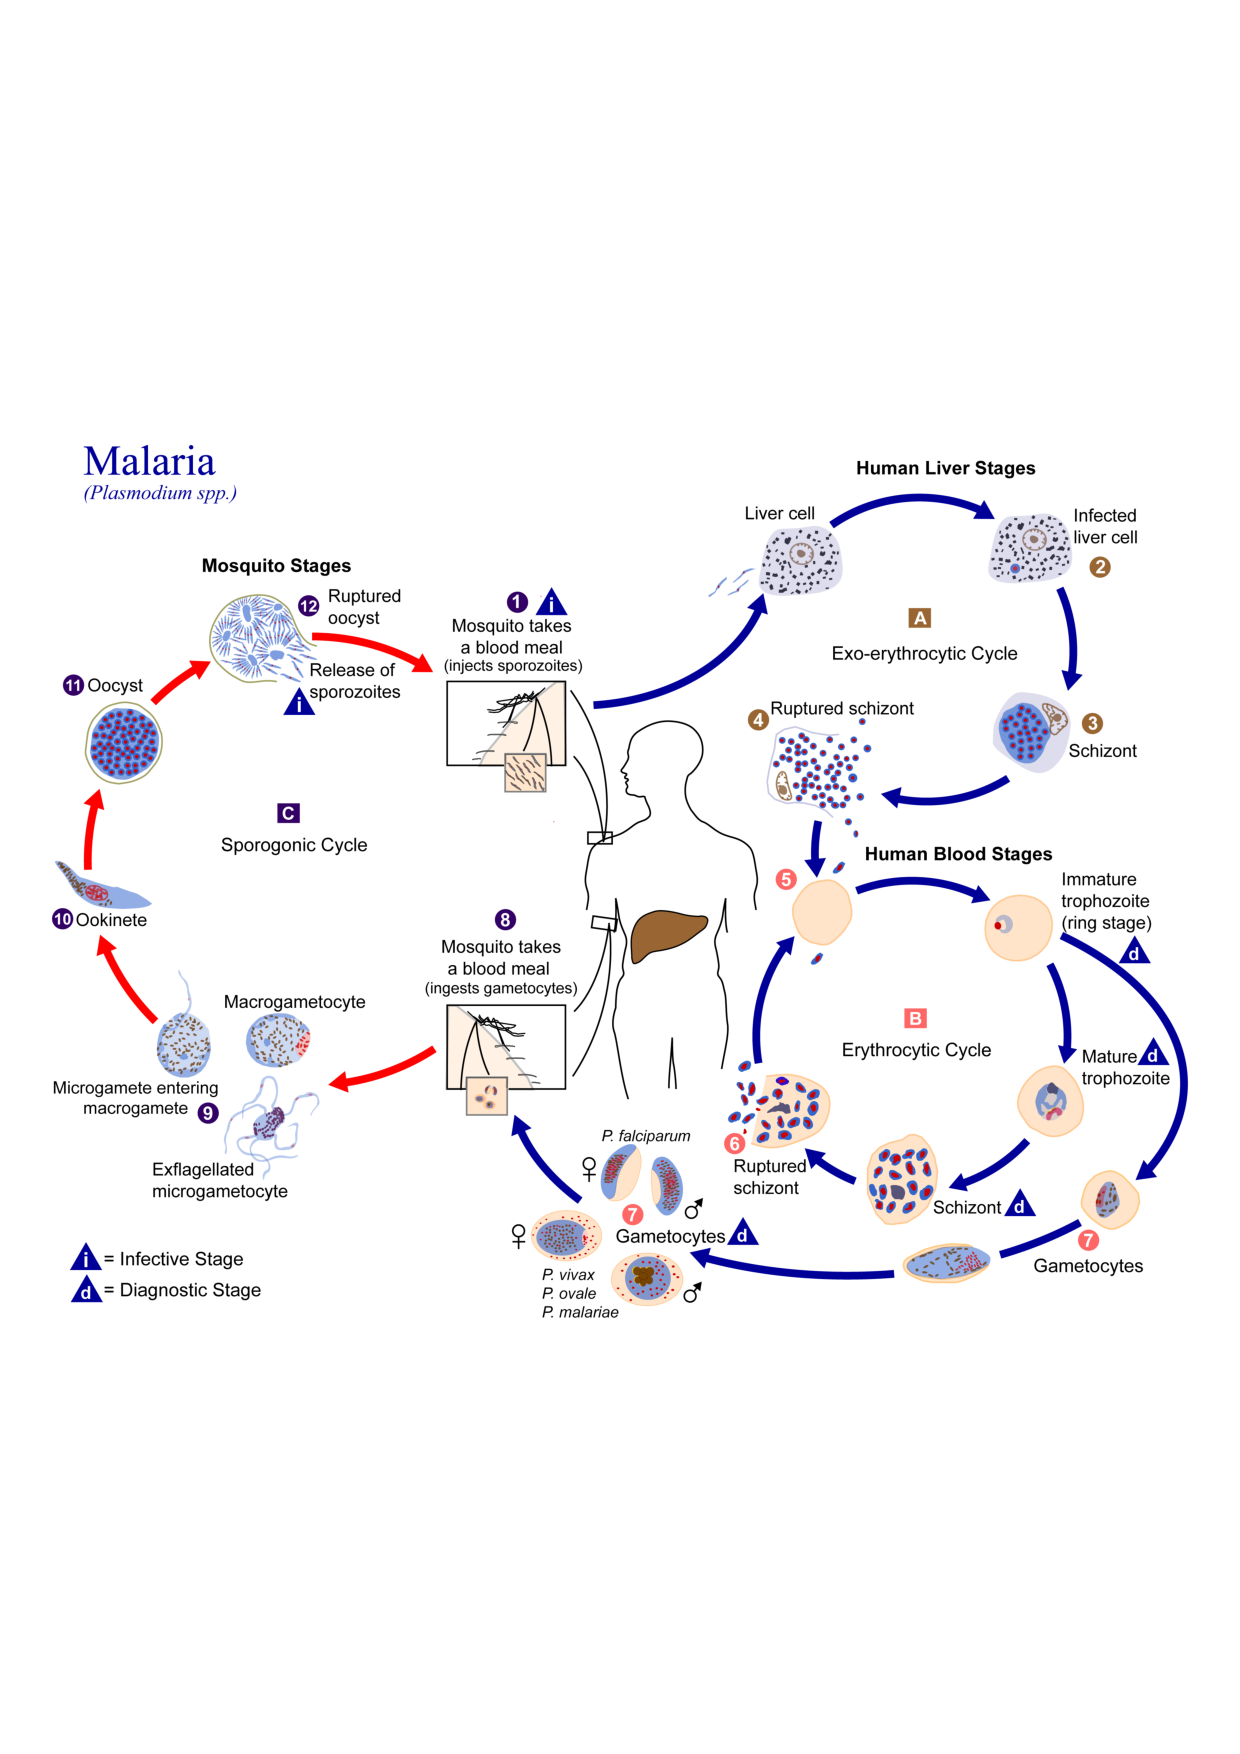
\includegraphics[width=0.9\textwidth]{lifecycle}
  \caption{Lifecycle of parasites from the \textit{Plasmodium} genus.  Reprinted from the CDC's public domain Public Health Image Library (PHIL), image \#3405.}
  \label{fig:lifecycle}
\end{figure}

\textit{Plasmodium falciparum} is a protozoan pathogen with a complex life cycle spanning several stages in (limited) vertebrate and mosquito hosts.  We shall review these stages and their constituent components in turn.

\subsection{Liver stage}

Vertebrate infection by \textit{P. falciparum} begins when a pregnant, infected \textit{Anopheles} spp. mosquito bites a host to consume a blood meal\cite{Ross:1897kh}.  Dozens to hundreds of \textbf{sporozoites} (the initial motile invasion stage of the \textit{falciparum} parasite) are transmitted to the host bloodstream via the saliva of the mosquito\cite{Amino:2006gj}.  The sporozoites travel the bloodstream until they reach the liver, infecting hepatocytes (specifically \textbf{Kupffer cells}: macrophages which express low levels of MHC I molecules\cite{Torre:2002bi}.

Inside the \textbf{parasitophorous vacuole} (a cytoplasm-filled protective envelope, "PV") produced by the sporozoite upon invasion of the hepatocyte, the parasite is protected from the phagolysosomes of the Kupffer cell and can begin asexual reproduction\cite{Lingelbach:1998us}.  The sporozoites undergo schizogonic development wherein the sporozoite produces many copies of its nucleus in preparation for multiple fission.  Upon cell segmentation, the parasite cells differentiate into \textbf{merozoites}, the next invasion stage of the \textit{falciparum} parasite.

The liver stage takes between $6$ and $8$ days\cite{Bousema:2014cy} to complete, producing thousands of haploid merozoites per parasetimized hepatocyte\cite{Prudencio:2006ho}.  This stage ends when the merozoites exit the hepatocytes and return to the bloodstream (presumably via physical rupture of the host cell).  
\subsection{Blood stage}

Newly released merozoites are non-motile; they come into contact with erythrocytes during transit in the bloodstream.  As erythrocytes are non-nucleated, thus lacking MHC I and II molecules, they make for an effective hiding place from the adaptive immune system\cite{Murphy:2011vw}.  Merozoites invade the RBCs quickly, within $60$ to $120$ seconds of their egress from hepatocytes\cite{Cowman:2006eu,Wright:2014ii} (presumably this speed is to minimize its exposure to immunological attack).  A merozoite once again forms a PV after invasion in order to create a more hospital development environment for itself.  This is followed by a repeating cycle of asexual reproduction.  The intra-erythrocytic development cycle progresses through three stages: \textbf{ring} (immature trophozoite, named for its morphology under microscopy), \textbf{trophozoite} (the merozoite after shedding its surface coat and invasion organelles in its apical complex), and \textbf{schizont} (a multi-nucleated cell resulting from multiple fission and just prior to cell segmentation)\cite{Josling:2015js}.  Eventually the schizont ruptures, releasing $16$ to $32$ merozoites into the bloodstream which can then quickly infect more erythrocytes.  This process takes $24$ to $48$ hours.

To avoid destruction in the spleen, the parasites express and transport to the surface of the parasetimized RBC (pRBC) a cytoadherence factor termed \textbf{PfEMP1} (\textit{Plasmodium falciparum} erythrocyte membrane protein $1$)\cite{Flick:2004fn}.  The pRBCs typically adhere to the endothelial cells of post-capillary vessels, thus withdrawing from peripheral circulation\cite{Fernandez:1998hn}.  Such parasites are said to be \textbf{sequestered} from the immune system, which affords the parasite time to replicate within the parasetimized cell.  Should the cell still come into contact with B-cells, each parasite's genome encodes approximately $60$ variants of this protein in a family of genes termed \textit{var}.  Little to no overlap exists in the repertoires of geographically distant parasites\cite{Zilversmit:2013jj}.  Expression of a single member of the \textit{var} gene famly is mutually exclusive with all other forms being silenced.  This differential expression is epigenetically controlled through the placement of methyllation marks on upstream promoter elements\cite{Jiang:2013bk}.

All clinical symptoms manifest during red blood cell rupture.  Waste products and toxic factors that accumulate in the cell are released into the blood stream when the cell is lysed.  This stimulates immune responses.  In uncomplicated malaria, symptoms include fever, chills, sweats, rigors, and other flu-like symptoms.  As many iterations of erythrocyte invasion, parasite replication, and erythrocyte rupture will occur, these symptoms can appear to periodically relapse.  Other symptoms such as anemia and hypovolemia may occur due to the destruction of RBCs.  Severe malaria may occur if the parasite sequestration occurs in the brain (\textbf{cerebral malaria, CM}), or in the placenta (\textbf{pregnancy associated malaria, PAM}), potentially compromising blood flow to critical tissues.  These severe pathologies are often fatal\cite{AlessandroBartoloni:2012gl}.

\subsection{Reproduction}

During the intra-erythrocytic development stage, approximately $10\%$ of parasites are randomly committed to developing into the sexual form: the \textbf{gametocyte}\cite{Sinden:1983tx}.  This is currently thought to occur in the erythrocytic schizonts.  Committed parasites reinvade new erythrocytes and mature into gametocytes in $10$ to $12$ days.  Mature gametocytes do not exit pRBCs within the human host.  Instead, they lie in wait for another mosquito to bite, drawing the gametocyte-carrying erythrocytes as part of the blood meal.  Gametocytes mature into male and female gametes upon sensing the different environmental conditions in the mosquito midgut (change in temperature, change in pH, and exposure to xanthurenate).  Mature haploid gametes fuse to form diploid zygotes, which soon matures into an \textbf{ookinete}, a motile form of the zygote that can penetrate the lumen of the mosquito stomach and in which meiotic recombination occurs.  The ookinete migrates to the mosquito mid-gut epithelial cell wall and forms an \textbf{oocyst}, a non-motile thick-walled spore on the exterior surface of the midgut.  The newly formed sporozoite replicates via mitosis within the oocyst.  The eventual oocyst rupture releases haploid sporozoites that migrate to the salivary gland of the mosquito.  Once the mosquito bites another host and transmits the new sporozoites, the cycle repeats.

\subsection{The \textit{P. falciparum} crosses}

Observing \textit{de novo} mutations in \textit{P. falciparum} parasites requires a system wherein we can obtain DNA for the new sporozoites and their progenitors.  Currently, no method for performing such crosses \textit{in vitro} exists, and using a human host for the vertebrate component of the parasite's life cycle would be ethically infeasible.  Rodent models are also inviable; \textit{Plasmodium falciparum} is very particular about its vertebrate hosts.  Only humans and our closest extant relatives, chimpanzees (\textit{Pan troglodytes}) are known to become infected.  In the latter case, it appears infection by \textit{P. falciparum} is asymptomatic, even in splenectomized chimpanzees with high levels of parasitemia\cite{MacFie:2009kn}.

All four crosses (3D7xHB3, HB3xDD2, 7G8xGB4, and 803xGB4) have involved infecting chimpanzees with sporozoites and later collection of pRBCs for later culturing and analysis\cite{RanfordCartwright:2012kp}.  Briefly, this protocol proceeds as follows.  First, gametocytes (3D7, HB3, DD2, 7G8, GB4, and 803) are cultured \textit{in vitro}.  Next, mosquitos are fed parasetimized blood through an artifical blood feeder\cite{Su:2007ipa}; hopefully the mosquitos ingest gametocytes from both parents.  These mosquitoes are then permitted to bite chimpanzees, passing the recombinant parasites (and non-recombinant forms as well, given that there is no mechanism to prevent self-crossings) to the animals' bloodstream.  Once blood-stage infection is detected, the parasites are harvested, cultured \textit{in vitro} (limiting dilutions ensure that each culture reflects a clonal expansion of a single sporozoite), and screened for recombinant progeny.  This process is repeated until enough recombinant progeny have been detected and successfully cultured.

Until single cell sequencing methods can recapitulate a cell's genome with extremely high fidelity, the culturing step is necessary to ensure adequate material for sequencing.  Most second-generation sequencing protocols require at least $1$ nanogram of DNA to proceed (though most recommendations call for much more), which is still tens of thousands of parasites required at minimum to ensure sufficient genomic yield during library construction.  PCR amplification is not recommended; high fidelty enzymes exhibit an error rate of $10^{-6}$ mutations/bp, which would lead to $230$ PCR-induced mutations in the $23$ megabase \textit{P. falciparum} genome.  Taken together, the need for culturing is clear.

However, culturing is a third environment in which the parasite must survive.  Culturing of \textit{Plasmodium} spp. parasites is notoriously difficult and laborious\cite{Schuster:2002ck}, and most parasites do not thrive in culture conditions.  Those that do almost certainly incur \textit{de novo} mutations that underlie culture adapation.  For example, the F12 line of parasites (derived from 3D7) is no longer capable of producing gametocytes\cite{Alano:1995gv,Gissot:2004dv,Silvestrini:2005gc}.  Almost certainly this is a response to existing exclusively in culture where the gametocytogenesis pathway cannot be completed.  Commitment to sexual differentiation would preclude further asexual replication in the committed parasites.  No selective pressure remains to ensure the genes involved in gametocytogenesis remain functional.  Parasites that do not produce gametocytes will quickly out-compete those that do.  Their new alleles will quickly reach fixation in the culture population, and many more might reach a nominal allele frequency in the pool.

The implications for what we can expect to see in second- and third-generation sequencing data are clear: we must expect mutations to appear with different allele frequencies, despite occurring in a seemingly haploid genome.  Any mutation sustained prior to mitosis of newly recombinant sporozoites in the ookinete will appear to be fixed in the sequenced sample.  As cultures are initiated with a single parasite (one hopes), any mutation sustained between recombination and harvesting from chimpanzee peripheral blood will also appear fixed.  Finally, mutations occurring \textit{in vitro} may or may not achieve fixation.  Barring reverse mutations, only \textit{de novo} mutations occurring during culture can ever be non-fixed in this experimental system.  Special care must be taken to not permit these mutations to confound rate calculations for mutational events in the genome, though future analyses regarding culture adaptation may do well to study them more carefully.

\section{Mutational types}

We have discussed the parasite life cycle which gives us a sense of when mutations may occur.  We now discuss the types of mutations we should expect to find, and the mechanisms that generate them.

\subsection{Point mutations}

Point mutations (single nucleotide variants, or SNVs) are the simplest (and likely most common) alteration that can occur in the genome.  These may be induced by exposure to mutagenic agents (ultraviolet radiation, oxidative damage, base analogs, alkylating agents, etc.).  More commonly, point mutations arise as the result of errors during DNA replication.  \textbf{Mispairings} between base pairs may occur when a nucleotide, capable of existing in various \textbf{tautomeric} forms (repositionings of a hydrogen atom which alters the hydrogen bonding pattern of the nuclotide) cause the altered form to bind to incorrect nucleotides.  Such a tautomeric shift may occur prior to or during replication without being corrected.  As the polymerase generates the compliment for each strand, the mispaired base opposite the tautometric base will have its true compliment incorporated, thus making the error permanent for all descendent cells\cite{Griffiths:2003wb}.

Similar replication errors may arise after \textbf{spontaneous base degradation}.  Deamination of cytosine (C) to uracil (U) - a non-standard nucleotide in the genome - can result in the mispairing between the latter and adenine (A).  Deamination of methylcytosine can produce a thymine.  Should these degraded nucleotides escape repair processes (and in the latter case, there is no error recognition mechanism to detect and remove the aberrant thymine, as it is a normal base in DNA), the changes will effectively be ratified by replication.

\subsection{Insertions, deletions, inversions}

The most common cause of \textbf{insertion} (the addition of one or more nucleotides to a locus in the genome) and \textbf{deletion} (the removal of one or more nucleotides) mutations is errors during the replication of repetitive elements.  This can occur when a repeat unit (or several) are looped out during replication, resulting in a "slip" in the template strand versus the nascent strand (an apparent insertion) or vice versa (an apparent deletion).

Indels also commonly arise as the result of DNA repair efforts on \textbf{double-strand breaks (DSBs)} by the cell, via a number of different repair pathways.  \textbf{Homology-directed repair (HDR)} proceeds by first resecting a short region around the DSB in the $5'$ to $3'$ directions on both strands.  A genome-wide homology search returns a (presumably) homologous template sequence with which to guide the repair.  \textbf{Strand invasion} brings the broken strands and complementary complete strands into proximity so that the missing sequence can be resynthesized, forming a DNA \textbf{heteroduplex}.  A \textbf{displacement loop (D-loop)} is formed between the invading $3'$ overhanging region and the homologous counterpart.  The action of the polymerase extends the invading $3'$ strand by synthesizing the missing sequence according to the template, and in doing so, the D-loop is changed to a cross-shaped structure known as a \textbf{Holliday junction}.  The crossing strands are cut, yielding the repaired chromosomes.  Mutations can arise if the homology search returns sequence that is similiar but not perfectly homologous to the lost sequence.  While in a diploid genome, the homology search would yield sequence on the sister chromatid, such a search necessarily yields a different part of a haploid genome.  Many types of mutation can be induced by this mechanism, including insertions, deletions, even inversions.

In contrast, \textbf{non-homologous end joining (NHEJ)} does not require a homologous template.  In most cases, a clean DSB (one that simply separates the strands at the same position in both strands) is easily repaired by the NHEJ pathway by simple ligation of the loose ends.  However, should the break be messier, a short region ($1$ to $4$ bp) around the DSB may first be resected in the $5'$ to $3'$ directions on both strands.  Once the ends are blunted and therefore compatible for ligation, the NHEJ pathway fuses the two loose ends, resulting in a deletion of the resected sequence\cite{Lieber:2008dn}.  In rare cases, the repair process can incorporate \textbf{non-homologous exogenous DNA} (free DNA that diffuses into the active site and gets caught in the repair process)\cite{HavivChesner:2007gm}.

The \textbf{microhomology-mediated end joining (MMEJ)} pathway also performs a lossy repair on double-strand breaks\cite{McVey:2008kp}.  Both strands are extensively resected until $5$ to $25$ bp homologies are located in each strand.  These homologous regions are annealed, leading to a deletion of everything between the DSB and the located homologies.  These deletions are substantially larger than those produced by NHEJ, typically from $30$ to $200$ bp in length\cite{Kent:2015jg}.

\textbf{Single-strand annealing (SSA)} can be employed to repair DSBs occurring between two repetitive sequences on the same strand with identical orientation\cite{Lin:1984uf}.  Single strand regions are created adjacent to the breaks via resection, extending to the end of the complimentary repeat sequence until the strands can be brought together by complementarity.  The $3'$ overhangs are then digested as necessary, and gaps are filled in the sequence in order to restore linearity.  The original sequence between the repeat copies is destroyed.

While in many genomes, \textbf{transposable elements} (DNA sequences that can move from one region of the genome to another) can contribute to indels, in the finished assembly of the \textit{Plasmodium falciparum} 3D7 reference genome, no transposable elements were found\cite{Gardner:2002p1564,Rebollo:2012js,Biemont:2006km}.

\subsection{Cross-overs}

Cross-overs can take place via \textbf{homologous recombination (HR)} during meiosis in the ookinete.  The process follows the steps outlined above for the HDR (although in the case of HR, the DSB is not the result of DNA damage, but rather is developmentally programmed to initiate the crossover).  The homology search now returns the homologous chromosome from the counterpart gamete.  Strand invasion and Holliday junction generation proceeds as usual so that the counterpart strand may be synthesized.  In contrast to HDR, the second $3'$ overhang (which was not part of the initial strand invasion) forms a second Holliday junction with the homologous chromosome.  Rather than cutting the Holliday junction on the crossing strands, two sets of cuts are made (one cut per junction): first on the crossing strand, the second on the non-crossing strands.  This results in the crossover product\cite{Sung:2006dk}.

While crossovers can produce new chromosomes not present in the gametes, the sequence immediately surrounding the breakpoint may not look altered.  Homologous recombination necessarily occurs in regions of homology.  In rare cases, the breakpoint may occur between two variants positions between the gametes and produce a crossover product that has the maternal allele on one end of the breakpoint and the paternal allele on the other.  Assembly-based approaches to variation discovery may miss this event unless the two alleles now appearing on the same haplotype also appear within a kmer length of one another.

\subsection{Gene conversion}

Gene conversions occur in the same manner as cross-overs, with one exception: should a sequence mismatch be present between the donor and acceptor strands in the heteroduplex, the mismatch must be repaired before the Holliday junctions can be resolved.  The mismatch repair process usually acts on the broken strand, using the intact strand as a template, thus effectively converting the sequnce of the broken strand to that of the intact strand in order to restore perfect complementarity.  The Holliday junctions are then resolved as they are for cross-overs, yielding a short stretch of sequence that appears to have been donated by one parent amidst the haplotypic background of another\cite{Chen:2007hb}.

Once again, these events are difficult to resolve in an assembly framework unless the mismatches are sufficiently close to one another.

\subsection{Non-allelic homologous recombination (NAHR)}

Occassionally, the genome-wide homology search during mitosis or meiosis may yield a template that is not an allele of the sequence being repaired.  In this scenario, the recombination machinery described above for cross-over and gene conversion events may yield a non-allelic repair.  This joins two disparate regions of the genome, often regions from non-homologous chromosomes, to produce a sequence absent from either parent.  Such \textbf{non-allelic homologous recombination (NAHR)} events are typically mediated by homologous repetitive elements: \textbf{segmental duplications, (SDs)}, typically $10$ to $300$ kb in length with $95\%$ to $97\%$ sequence identity among them\cite{Gu:2008jl,Sasaki:2010bm,Roehl:2010bt,Parks:2015hj}.  The SDs from different regions of the genome are brought together in the cross-over pathway to generate the new sequence.  As it is unlikely that these regions are perfect homologs, the additional action of mismatch repair may generate some additional sequence modifications before the final sequence is synthesized.

Identification of NAHR events in assembly data is non-trivial.  In a perfect assembly, one should be able to observe repeated template switching of the child's haplotype to the maternal and paternal haplotypes, and additionally detect that the templates do not belong to the same locus.  However, as NAHR events are mediated by homology, the assembly must be able to overcome the resultant loops in the graph without ambiguity in order to complete the traversal.  This is unlikely to be achieved every time (if ever).  Thus, in second-generation sequencing data, one expects an NAHR event to manifest as multiple pieces.

The \textit{P. falciparum} genome is $80\%$ AT, highly repetitive, and contains a number of highly conserved SDs in subtelomeric regions of several chromosomes\cite{Mok:2008ja}.  Notably, the subtelomeric regions of nearly all of \textit{P. falciparum's} $14$ chromosomes (excluding the mitochondria and apicoplast) house several members of the antigenic gene families, \textit{var}, \textit{rifin}, and \textit{stevor}.  As mitotic diversification of the \textit{var} genes has been observed many times, NAHR is thought to be a critical capability of a pathogen that must continuously evade immune pressure to survive.

\section{Known rates}

Little work has been done on \textit{de novo} mutation rates in \textit{P. falciparum}.  Two studies are known to exist: both using clone trees of selected parasites.

Bopp \textit{et al.} investigated parasite genome changes over time by generating new cell lines from the 3D7 parasite and DD2 parasites.  The authors reported detection of $167$ SNVs in $25$ clones total ($6.68$ SNVs per sample on average) and $59$ structural variants (insertions and deletions).  Bopp \textit{et al.} estimate the SNV rate to be $1.7-3.2 \times 10^{-9}$ mutations per base per generation (absent clones exposed to anti-malarial drugs), and $9.5 \times 10^{-6}$ structural variations per base per generation\cite{Bopp:2013gr}.  SNVs were relatively confined to the so-called \textbf{core} of the genome (excluding subtelomeric, pericentromeric, and interspersed hypervariable regions), while structural variants were found predominantly in subtelomeric regions housing antigenic genes.

Claessens \textit{et al.} find similar numbers in their clone tree work.  Having produced and whole-genome sequenced $37$, $56$, and $81$ subclones from the 3D7, DD2, and HB3 (respectively), the authors find SNV mutation rates of $4.07$, $3.63$, and $3.78 \times 10^{-10}$ mutations per base per generation\cite{Claessens:2014fo}.  While this may seem considerably different than the Bopp \textit{et al.} estimate, the Bopp estimates adjusted their raw data to account for non-synonymous deleterious mutations that may have been eliminated by purifying selection prior to identification.  Adjusting the Claessens \textit{et al.} estimates using the Bopp methodology, the rates become $4.28$, $3.82$, and $3.98 \times 10^{-9}$, in line with the Bopp estimates.  Claessens \textit{et al.} note that they observed "back-to-back" mutations (what we refer to in this dissertation as \textit{multi-nucleotide polymorphisms, MNPs}).  In their rate calculations, they considered these as two adjacent SNPs, but note that this assumption may be unwarranted.

In examining NAHR, Claessens \textit{et al.} isolated their analysis to exon $1$ of \textit{var} genes in 3D7, DD2, and HB3.  This is the longer exon of the two that comprise \textit{var} genes, and encodes the region of the PfEMP1 protein that is immunologically exposed.  The authors report a ratio of exon $1$ recombinations per SNP to be $0.27$, $0.35$, and $0$ for 3D7, DD2, and HB3, respectively.  HB3 is notable in that it appears to exhibit no NAHR events whatsoever.

\section{Biases}

In humans and chimpanzees, it has been shown that the \textit{de novo} mutation rate in the children is largely driven by the age of the father at conception\cite{Kong:2012ek,Venn:2014ep}.  From five months prior to birth to birth itself, female primordial germ cells undergo a mere $22$ mitotic divisions, and $2$ meiotic divisions during sexual maturity\cite{Crow:2000gn} to produce mature female gametes (ova).  In contrast, male sperm stem cells undergo a division every $16$ days in addition to subsequent mitotic divisions of the gonial cells ($4$) and meiotic divisions of the meiotic cells ($2$).  The sperm cells thus have vastly more opportunities to accumulate errors than ova.  A number of disorders (e.g. Apert syndrome, achondroplastia, thanatophoric dysplasia, Costello syndrome, etc.) have been associated to \textit{de novo} mutation\cite{Glaser:2003da,Goriely:2012fi,Veltman:2012gw}.

In \textit{P. falciparum}, no information regarding a parental age effect is available.  The experiment would be exceedingly difficult to perform in principle as we'd have to ensure that one parasite only contributed male gametocytes and the other only contributed female gametocytes.  In our crosses, the "gender" of the parents may change from one progeny to the next; no data is available for the gender of the gametocytes that have contributed their genetic material to the resulting progeny.
